%! Author = cspiller
%! Date = 17/11/2022

\thispagestyle{plain}
\newpage
\section{Project Plan}\label{sec:project-plan}

\normalsize

Following from the first phase of the development cycle the plan for the project was refined in light of the information that was gathered.
The processes for communication were also refined, alongside revised plans as to what tasks the project required.
There also followed some consideration of what resources were required to fulfill the project requirements.

\subsection{Timeline}\label{subsec:timeline}

The below series of figures (\ref{fig:timeline1},~\ref{fig:timeline2},~\ref{fig:timeline3}) detail the updated development tasks, and the planned timeframes for completion.
Timeframes were adjusted in accordance with the perceived complexity of each task following enlightenment from the literature review and market research.
Dependencies for each task were also calculated and can be seen as arrow representation in the timeline figures.

\begin{figure}[!htb]
    \minipage{\textwidth}
    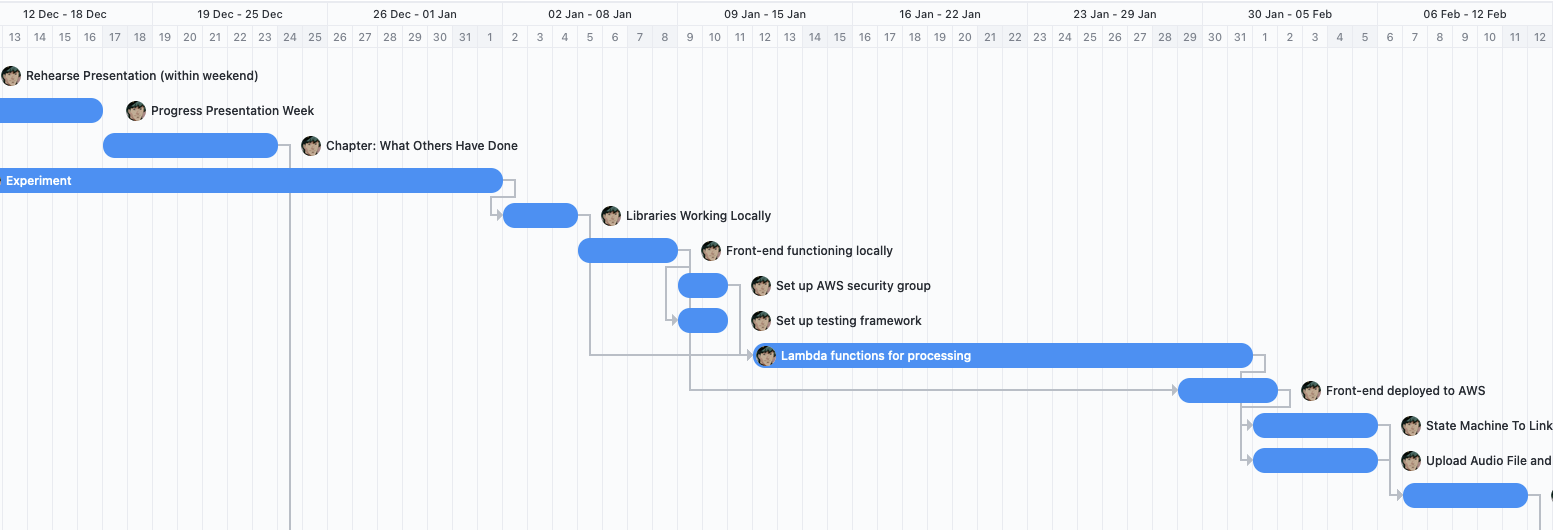
\includegraphics[width=\linewidth]{timeline1}
    \caption{Timeline: $Dec~12th~\rightarrow~Feb~12th$}\label{fig:timeline1}
    \endminipage\hfill
    \minipage{\textwidth}
    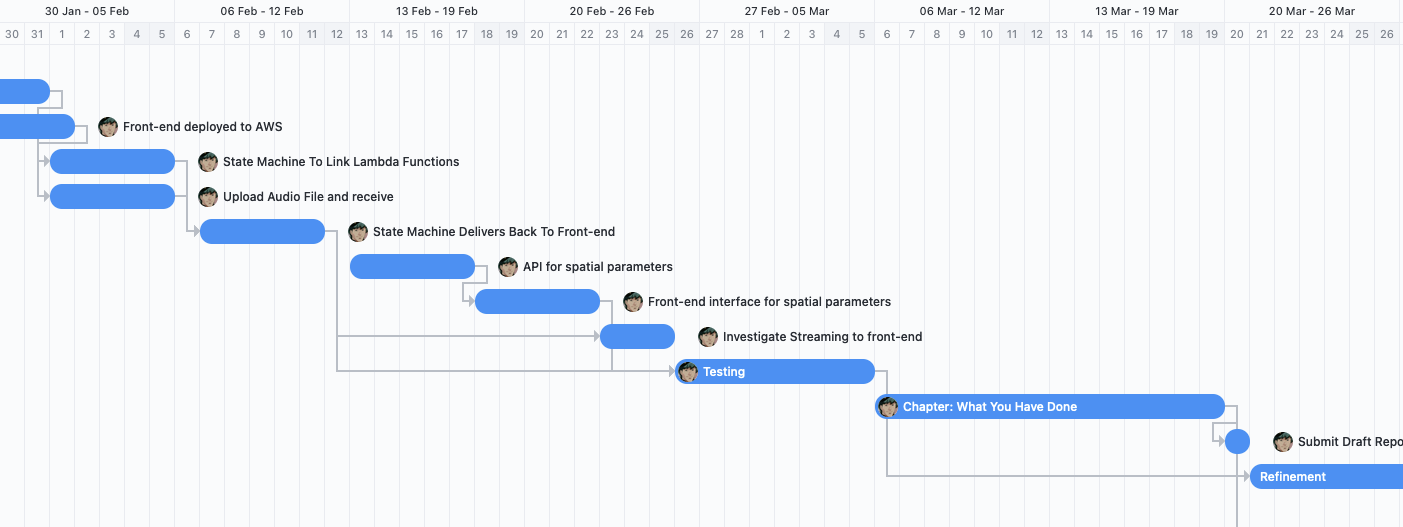
\includegraphics[width=\linewidth]{timeline2}
    \caption{Timeline: $Jan~30th~\rightarrow~Mar~26th$}\label{fig:timeline2}
    \endminipage\hfill
    \minipage{\textwidth}
    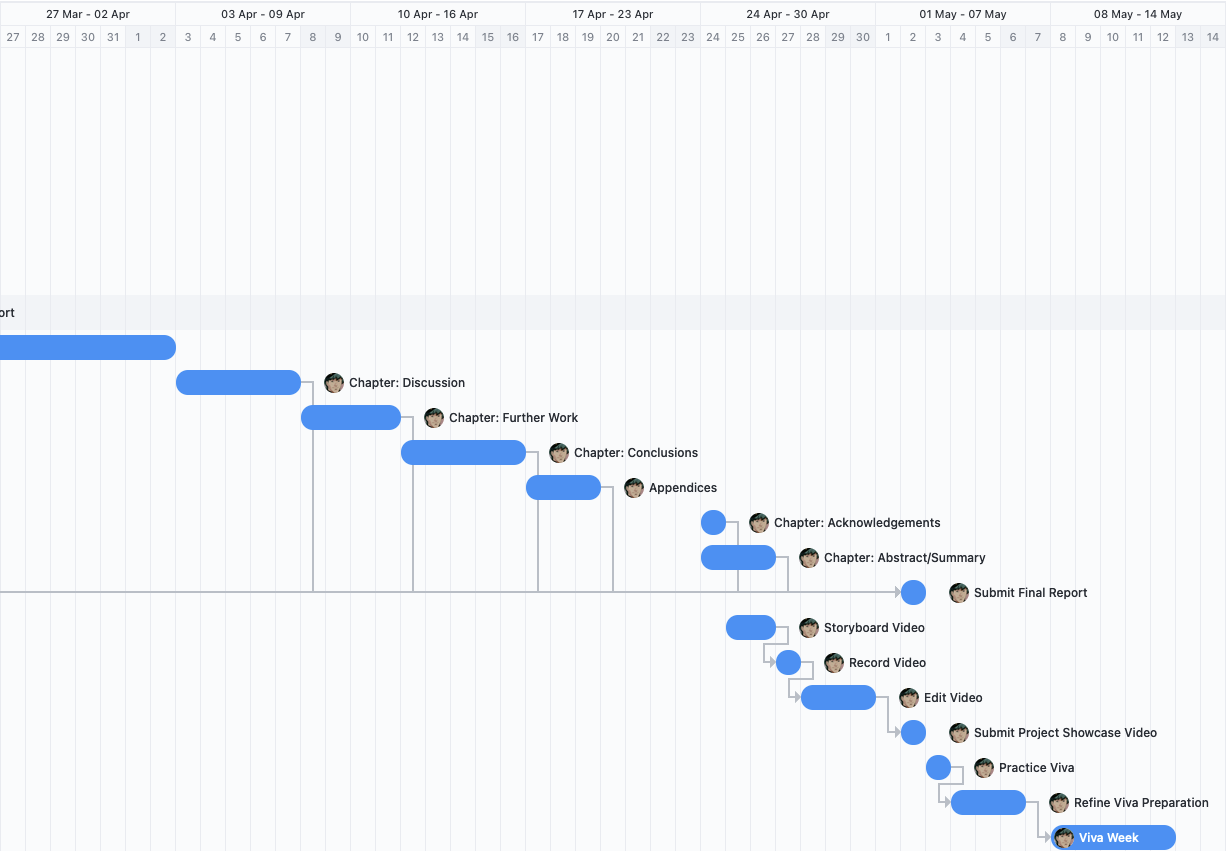
\includegraphics[width=\linewidth]{timeline3}
    \caption{Timeline: $Mar~27th~\rightarrow~May~14th$}\label{fig:timeline3}
    \endminipage
\end{figure}

\subsection{Communication}\label{subsec:communication}

This project makes use of the ClickUp\footnote{\citep{clickup}} software to perform project management functions and to organize this author’s workflow.
This software has been chosen over other pieces of software in the education\footnote{\citep{education_software}} and project management\footnote{\citep{pm_software}} space on the basis of cost and ease-of-use, as well as its ability to synchronize across platforms.
In addition, the platform will also be used to communicate with the project supervisor who is able to see the project plan and its progress over time.

Prioritizing communication with the supervisor is integral to the success of the project because of the accountability and oversight it provides to this author.
Having a platform such as ClickUp drastically reduces the likelihood of error in communication and time management.

\subsection{Resources}\label{subsec:resources}

This project intends to use minimal resources in its development.
As outlined in~\ref{sec:literature-review}, one of the many advantages of cloud computing is its flexibility and ease of resource management.
Given that the application will be hosted entirely in cloud environments, there will be no hardware costs associated with the project.
The costs that do apply will relate to the use of the~\gls{aws} platform.
These costs must be managed carefully, as explained in~\ref{subsec:business-risks}.

Other resources utilized will include:

\begin{enumerate}
    \item Queen Mary library resources
    \item The project supervisor
    \item Knowledge sharing from colleagues at~\gls{sie}
    \item JetBrains’~\gls{ide} Suite
    \item Open-source audio-processing libraries.
\end{enumerate}
